\renewcommand\TheFile{intro.tex}
\SVN $Author: hom $
\SVN $Revision: 14 $
\SVN $Id: intro.tex 14 2013-05-13 13:36:54Z hom $
\SVN $Date: 2013-05-13 15:36:54 +0200 (Mon, 13 May 2013) $
\SVN $State: Exp $

\begin{savequote}[8cm]
  \sffamily
  What's up doc?
  \qauthor{Bugs Bunny}
\end{savequote}
\chapter{Module description}
\section{Goal}
\parpic(42mm,32mm){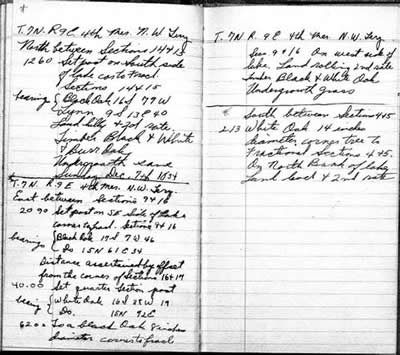
\includegraphics[width=40mm]{figures/INT082E06-description4.jpg}}
The students achieve competences in specifying, analysis and design of
a reactive system with hardware control, using UML and in implementing
this system in Java.

The application of Design Patterns is stimulated. The concrete
elevator modelling is a good exercise in thinking about and applying
design rules that have been studied in the previous module Modelling~2.

\subsection{Goal in accordance with Dublin Descriptors}
The module addresses all 4 of the 5 Dublin descriptors as follows:
\begin{Itemize}
\item \textbf{Demonstrate the knowledge and understanding} by applying
  \textit{UML}, \textit{Analysis and Design Rules} and \textit{Design
    Patterns} to Analysis and Design of a moderately complex system; 
\item \textbf{Apply the knowledge and understanding} in the
    Implementation of a moderately complex system;
  \item \textbf{Identifies and uses data to formulate responses} by
    Analysing the system to be designed;
  \item \textbf{Communicates about understanding, skills and
      activities} by means of a report;
\end{Itemize}

Of the ICT specific competences the following are addressed:
\begin{Itemize}
\item Analysis
\item Design
\item Realisation
\end{Itemize}

%\vspace{30mm}

\subsection{Explanation and  content}
The project task is as follows:
\begin{Enumerate}
\item Create a detailed analysis and design of the system using
  UML models. The implementation should include a hardware controlling version
  and a graphical simulation. It should be possible to run the program
  without having the hardware system available.
\item The UML model should be created using Visual Paradigm. We
  expect the following artefacts in the models: Use Case diagram
  including Use Case descriptions, CRC cards for the classes to be
  implemented, sequence diagram for the main scenarios and state
  diagrams for the reactive components.
\item Implementation and test of this system using Java and the
  IO-warrior kit to connect the hardware system to the computer.
\item Implementation and test of a GUI simulation of an elevator
  system in Swing.
\end{Enumerate}


\subsection{Learning goals}
Learning goals:

The student is able to apply UML to an analysis and design problem for
a  system with a graphical and a reactive aspect in a program of
medium complexity.

The student is able to implement a program with graphical elements and
a simulation.

The student is able to programmatically control hardware. 

To start a glance at Head First Object Oriented Analysis and Design
\cite{HFOOAD} is worth while. In particular keep the advice in chapter
8 in mind.
In the previous MOD2 module the students learned how to understand and
apply patterns in theory using the book Head First Design Patterns \cite{HFDP}.
As additional reference the Gang of Four patterns book \cite{GOF} can
be used for patterns not fully covered in \cite{HFDP}. \Code{Builder}
is of particular use in this project.

For aspects dealing with state behavior \cite{DHT} provides a useful
background. 

Grading is determined by the next table, showing the weights of the various aspects.

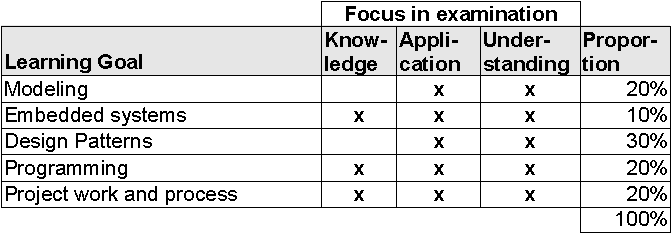
\includegraphics{tables/learninggoals-crop.pdf}


\paragraph{Previous modules} MOD1, SEN1, PRO1 and PRO2, PRJ31, MOD2.
All modules mentioned are mandatory.

\paragraph{Time planning} The time plan of the module during the
course weeks is summarised in the table below.

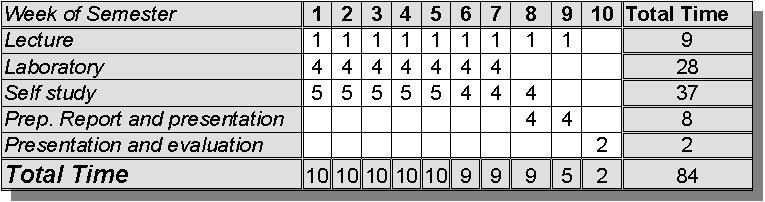
\includegraphics{tables/timetable-crop.pdf}


\subsection{Grading}
This is a group project. The grade of the individual will depend on
the group grade, the peerweb peer assessment and the individual
evaluation by the tutor.

\subsection{Project hard- and software requirements}
Each group should have access to an elevator system with a USB
connector. This setup allows the connection to any system supporting
USB and Java. This includes Windows XP, Vista and 7, Linux in all its
distributions and MAC OS-X. The USB adapter can be used safely in
connection with any laptop.


